\chapter{基于分区信道建模的回读信号生成 \label{sec:chapter.cnn1}}
	本章针对回读信号区分度不足的问题，提出解决方案。首先，分析传统均匀信道模型在高密度条件下的局限性。接着，详细阐述基于点扩散函数（PSF）的多分区建模方法，包括分区策略、各分区简化响应函数的构建过程。最后，通过仿真实验，验证所提模型在信号匹配精度和计算效率方面的优势，并与传统模型进行对比分析。

\section{现有回读建模方法及其局限性分析}

为实现高密度AD光盘信号的高性能均衡，首先需要构建一个能够精确表征其信道特性的回读模型。一个理想的模型应同时满足高仿真精度与高计算效率的双重要求，为后续自适应均衡算法提供充分且可靠的数据基础。

传统的信道建模主要分为两类：基于信号处理框架的简化线性模型与基于物理光学原理的衍射模型，二者在应对高密度、多维干扰场景时均存在明显局限。

常用的Bergmans线性模型[\textcolor{red}{插入文献}]是基于信号处理框架的简化线性模型。该模型将光盘信道简化为一个线性时不变系统，其冲击响应  $f(t)$  通常由高斯函数等形式描述（如公式\ref{eq.bergmans1}），读出信号 $h(t)$  视为 \( f(t) \) 与记录符矩形脉冲 \( c(t) \) 的卷积，如公式\ref{eq.bergmans2}。

\begin{align}
	f\left( t \right) &= \frac{2\sqrt{2}}{ST\sqrt{\pi}} \exp\left\{ -2 \left( \frac{2t}{ST} \right)^{2} \right\},  \label{eq.bergmans1} \\
	t_0 =  \frac{0.86\lambda}{NA} , \label{eq.t0} \\
	h(t) &= f(t) * c(t), \label{eq.bergmans2}
\end{align}

其中，T 是通道符号位周期，即比特位长度， S 是归一化信息密度，反映
了码间串扰（Intersymbol Interference, ISI）强度。$S = 𝑡_0/T$，$𝑡_0$ 是入射光斑最强
的$1/e^2$处的光斑直径，其计算公式如式\ref{eq.t0} 。该模型结构简洁，计算效率高，便于集成到均衡与检测算法中进行快速仿真。然而，其模型参数（如归一化信息密度 \( S \) ）本质上是经验性的，无法反映信道畸变背后的物理机理。当应用于更高密度、窄轨距的AD光盘时，模型无法准确刻画由光学衍射、像差及轨道间耦合效应引起的复杂空间变化特性，导致其生成的训练数据与真实信道响应之间存在失配，制约了均衡器性能上限。

另一种常用的Braat-Hopkins模型[\textcolor{red}{插入文献}]是基于物理光学原理的衍射模型。该模型从标量衍射理论出发，严格推导了光学系统的频率响应（如式\ref{eq.frequency}所示），

\begin{align}
	F\left( \frac{\Omega}{\Omega_t} \right) &= 
	\begin{cases} 
		\frac{2}{\pi} \left[ \arccos \left( \left| \frac{\Omega}{\Omega_t} \right| \right) 
		- \left| \frac{\Omega}{\Omega_t} \right| \right] \sqrt{1 - \left( \frac{\Omega}{\Omega_t} \right)^2 } \text{J}, 
		& \left| \frac{\Omega}{\Omega_t} \right| < 1 \\[8pt]
		0, 
		& \left| \frac{\Omega}{\Omega_t} \right| \geq 1 
	\end{cases}, \label{eq.frequency} \\
\end{align}
\begin{align}
\Omega_{\epsilon} &= \frac{2NA}{\lambda}\, T_c, \label{eq.omega_epsilon} 
\end{align}

其截止频率 \( \Omega_c \) 直接由激光波长 \( \lambda \)、物镜数值孔径 \( NA \) 等物理参数决定（式\ref{eq.omega_epsilon}）。该模型物理意义清晰，能够从本质上解释ISI的产生及光学系统的带宽限制，是光学头设计的理论基础。然而，其完整的数值计算涉及复杂的积分与变换，计算开销巨大，难以用于需要海量数据迭代的自适应均衡算法训练，工程实用性受限。

综上所述，Bergmans模型与Braat-Hopkins模型，二者均难以独立满足高密度AD光盘均衡研究对信道模型精准高效的要求。因此，本文在继承Braat-Hopkins模型物理内核基础上，提出一种多分区建模策略。该策略旨在将物理光学原理与工程可计算性相结合，通过将全盘信道划分为多个特征子区，并为每个子区构建兼具物理可信度与计算轻量化的响应函数，从而生成更贴合高密度AD光盘实际、更能反映区域差异性的高质量均衡信号数据集，为后续多通道自适应均衡技术的有效实施奠定坚实的模型基础。

\section{基于PSF的回读响应函数构建}
光学信息存储系统的读出过程，本质上是扫描成像问题。其核心物理模型描述了聚焦光斑与信息微结构（如光盘的信息坑）相互作用，最终在探测器上生成电信号的过程。

Braat与Hopkins等人的经典工作，为分析这一过程建立了严格的理论框架。他们基于标量衍射理论和部分相干光理论，将光盘读出系统精确建模为一类共焦扫描光学显微镜【文献 Book of Diffractive read-out of optical discs 】。尽管这一理论模型在物理上极为完备，但其计算形式复杂，需通过求解一系列衍射积分或级数展开来完成，难以直接用于需要快速评估大量数据图案的工程仿真中。

为满足高密度AD光盘存储系统中对复杂编码方案及信道性能进行高效、大规模仿真的需求，一种广泛应用的工程化近似模型应运而生。该模型直接基于点扩散函数（Point Spread Function， PSF）【文献 2020_(Kimihiro Saito)_Optical disc writing strategy for analog signal recording】，将读出过程简化为一个空间卷积运算，在保证物理本质正确的同时，极大提升了计算效率。

在本研究中，采用基于理想衍射极限条件的PSF模型来描述光学探头在信息层上的光强分布\textcolor{red}{这里插入那个PSF的图，自己重新画}。当系统无像差且完美聚焦时，圆形光瞳所成的聚焦光斑强度分布，即PSF，可由艾里斑（Airy Pattern） 的强度公式精确描述：

\begin{equation}
	\text{PSF}(x, y) = I_0 \left[ \frac{J_1(\bar{r})}{\bar{r}} \right]^2, \label{eq.psf}
\end{equation}

其中，

$\text{PSF}(x, y)$：表示在信息层平面上，以光斑中心为原点，坐标为$(x, y)$处的归一化光强分布。

$I_0$：峰值光强，与入射激光功率成正比，在归一化模型中常取为1。

$J_1(\cdot)$：第一类一阶贝塞尔函数。其振荡特性决定了艾里斑的主瓣与外围衍射环的结构。

$\bar{r}$：归一化径向坐标，其定义为：
\begin{equation}
	\bar{r} = \frac{2\pi \cdot NA}{\lambda} \sqrt{x^2 + y^2}
\end{equation}

$NA$：物镜的数值孔径，是决定系统分辨率的核心参数，$NA = n \sin\theta$，其中$n$为物镜与盘片间介质的折射率，$\theta$为物镜的半孔径角。

$\lambda$：激光在真空中的波长。

该公式具有明确的物理意义：$\lambda/NA$ 表征了系统的特征衍射长度。艾里斑主瓣的半高全宽（FWHM）约为 $0.51\lambda/NA$，这直接定义了光学系统所能分辨的最小空间特征尺度。

基于此PSF模型，探测器在扫描过程中接收到的瞬时光强信号 $S(t)$，可建模为PSF与盘片上反射率（或相位）分布 $R(x, y)$ 的卷积在光斑扫描轨迹上的积分：

\begin{equation}
	S(t) = \iint_{\text{扫描区}} \text{PSF}(x - vt, y) \cdot R(x, y)  dxdy , \label{eq.st}
\end{equation}

其中，$v$ 为扫描线速度，$R(x, y)$ 由记录的信息标记（如相变材料的晶态/非晶态区域）图案决定。此模型将复杂的衍射过程，转化为直观的空间滤波操作：PSF作为系统的空间冲击响应，对信息图案进行低通滤波，其截止频率即由 $\lambda$ 和 $NA$ 决定。

因此，基于艾里斑的PSF模型，成功地将Braat-Hopkins理论中的核心物理（衍射极限分辨率）封装于一个简洁的数学表达式中，为后续进行高效、可扩展的多分区回读信道建模与性能仿真奠定了坚实的基础。

\textbf{（1）光学头分区策略与特征提取}

光学读出系统的空间采样特性直接影响回读信号的多样性与信息容量。传统光学存储系统通常采用单一、对称的光学探头设计，其探测光斑在跨道（Radial）与沿道（Tangential）方向上的响应相对固定，限制了从光斑衍射场中提取多维度信道状态信息的能力。为应对高密度记录下日益严重的道间串扰与符号间干扰，本文借鉴先进磁记录系统中的空间分集采样思想，提出了一种新型光学头分区策略，旨在通过结构化、差异化的光场采样，提取具有空间相关性的多通道回读信号，为后续联合信号处理提供基础。

现有技术\textcolor{red}{插入专利文献}中采用的一种典型光学头分区模式（记为P0）如图\ref{fig:ch.cnn1.Pattern_P0} 所示。该模式将光学头有效孔径在归一化坐标系下划分为六个独立的探测区域，各分区中心在空间上对应于光斑的不同采样位置。这种设计的核心思想是利用光瞳平面上的空间分割，从单个聚焦光斑的衍射场中同时提取多个具有位置差异的信号分量。

\begin{figure}[h]
	\centering
	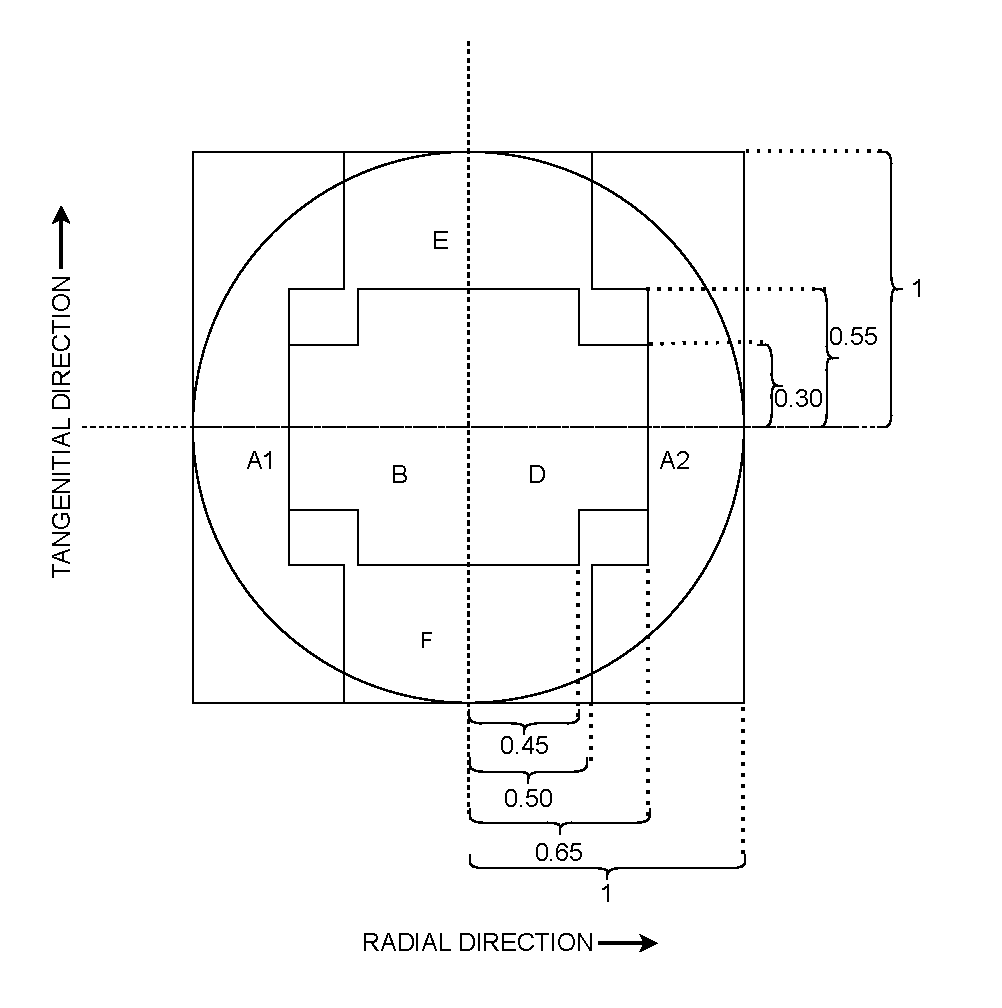
\includegraphics[width=0.6\textwidth]{float/ch.cnn1/Pattern_P0.pdf}
	\caption{光学头P0分区模式\label{fig:ch.cnn1.Pattern_P0}}
	% \setlength{\belowcaptionskip}{-10pt}
\end{figure}


尽管P0分区模式引入了空间分割，但其分区策略主要服务于传统的聚焦与跟踪伺服控制，对于从信号处理角度最大化空间采样多样性、以抑制高密度下的二维干扰而言，仍有优化空间。受二维磁记录（Two-Dimensional Magnetic Recording, TDMR） 技术的启发，本论文提出了一种面向联合信号处理优化的新型光学头分区模式（记为P1），如图\ref{fig:ch.cnn1.Pattern_P1}所示。
\begin{figure}[h]
	\centering
	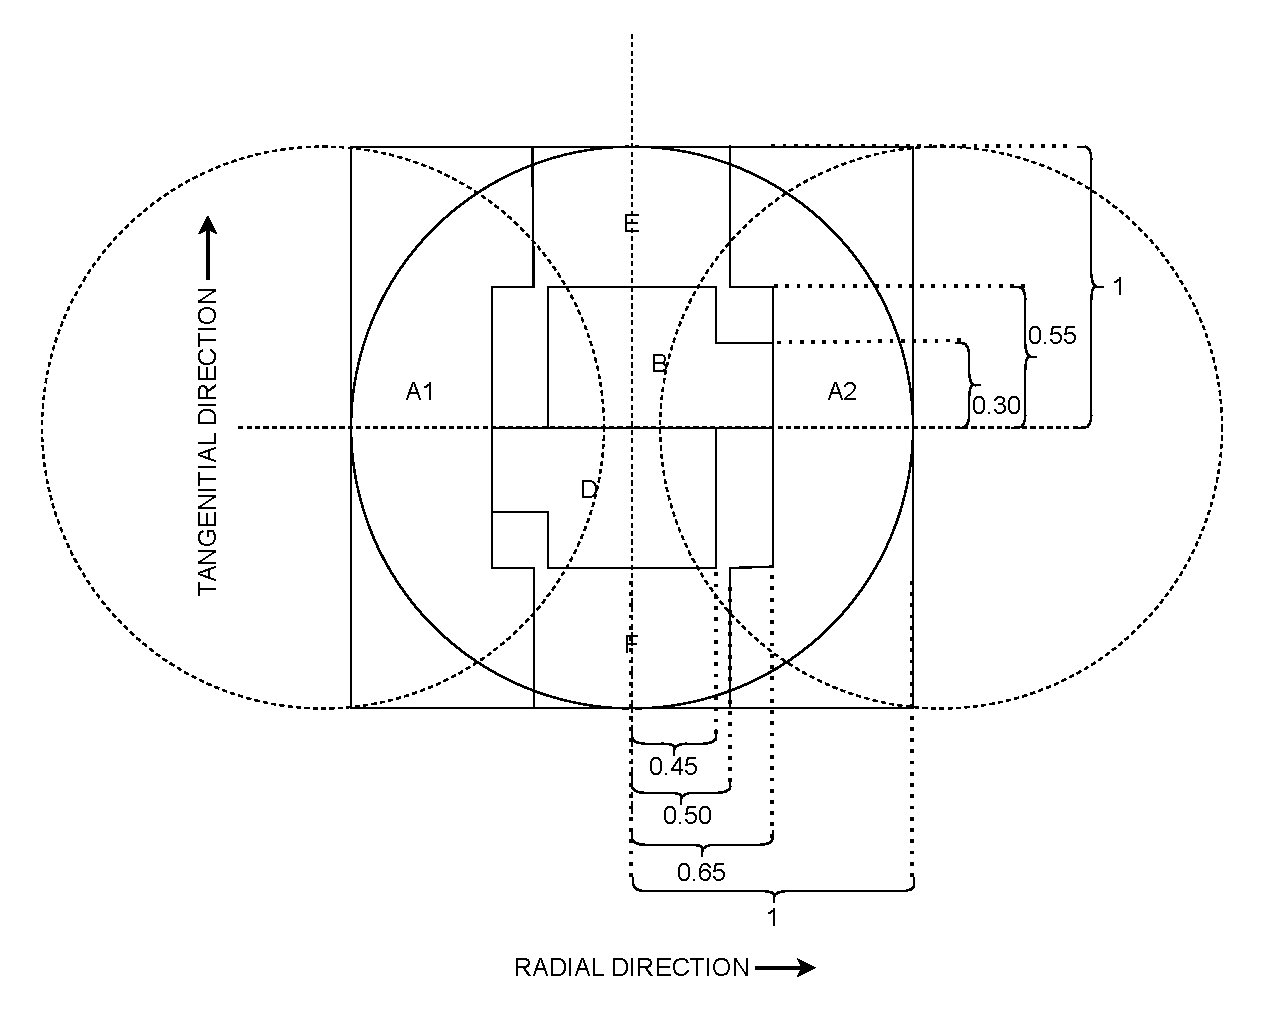
\includegraphics[width=0.8\textwidth]{float/ch.cnn1/Pattern_P1.pdf}
	\caption{光学头P1分区模式\label{fig:ch.cnn1.Pattern_P1}}
	% \setlength{\belowcaptionskip}{-10pt}
\end{figure}
TDMR技术是应对硬盘存储面密度极限的关键方案之一。在TDMR系统中，为了有效读取因磁道极度狭窄而重叠的磁化图案，采用了双读磁头或多读传感器阵列\textcolor{red}{插入文献}。这些传感器在跨磁道方向上具有微小的位置偏移，从而对同一数据位在相邻磁道上的“印记”产生不同的响应。通过同时采集这些空间位置各异的信号，并送入一个多通道联合均衡器进行处理，可以显著抵消道间串扰，恢复出原本无法可靠读取的数据。

借鉴这一思想，本设计认识到：光学头各分区在跨道方向上的相对位置差异，是产生信号多样性、从而对抗道间串扰的关键资源。因此，P1模式继承P0模式中A1、A2、E、F的基本布局，主要对B和D这两个关键分区的边界位置与形状进行重新设计，设计目标是要使这两个分区对同一信息位，因其在相邻轨道上的空间扩展（即比特轮廓）而产生的不同感应最大化。换言之，当光斑扫过一个信息标记时，由于道间串扰，标记在相邻轨道上的“拖尾”会被B区和D区以不同的权重感知，新设计的分区边界需要体现这种感知的差异性。与P0相比，P1中B与D分区的边界更加精细，其非对称性可能更加显著或经过特定调整，能更精确地体现出跨道方向上的信号差异。


\textbf{（2）分区响应函数构建}

为将前述理论模型应用于 P1 新型光学头分区模式，需要对聚焦光斑与信息标记相互作用后的衍射光场进行空间选择性积分。本文将 P1 分区中第 \( k \) 个区域（\( k \in \{A1, A2, B, D, E, F\} \)）的瞬态响应函数 \( S_k(t) \) 定义为：

\begin{align}
	\text{PSF}_k(x, y) = I_0 \left[ \frac{J_1(\bar{r})}{\bar{r}} \right]^2 \cdot H_k(x,y), \label{eq.psf_k} \\ 
	S_k(t) = \iint \text{PSF}_k(x - vt, y) \cdot M_k(x, y) \, dx dy,
	\label{eq.channel_response_simplified}
\end{align}

其中，\( \text{PSF}_k(x, y) \) 是分区 \( k \) 在公式\ref{eq.psf}上做空间选择积分得到的对应的有效点扩散函数。$H_k(x,y)$分区$k$的几何孔径函数。这是一个二值函数，在光瞳平面上对应分区 
$k$所覆盖的区域内取值为 1，否则为 0，此函数是 P1 分区模式硬件特征的直接数学表征。


\section{基于分区的多通道回读信号生成}
本节生成多分区回读信号数据集，以直观展示各通道的信号特征。数据经过 PCWA110 调制编码后写入光盘，实验条件设定为AD500光盘通道参数如\ref{tab:simulation_parameters}表。

\begin{table}[h]
	\centering
	\caption{AD500光盘系统仿真参数}
	\label{tab:simulation_parameters}
	\begin{tabular}{ll}
		\toprule
		\textbf{参数} & \textbf{数值} \\
		\midrule
		激光波长 ($\lambda$) & 405 nm \\
		数值孔径 ($NA$) & 0.91 \\
		最小标记长度 & 68.4 nm (34.2 nm/T) \\
		轨道间距 (Track Pitch) & 0.225 $\mu$m (225 nm) \\
		标记宽度 (Mark Width) & 133 nm \\
		记录方式 & TL/side $\times$ 2 sides \\
		\bottomrule
	\end{tabular}
\end{table}

\begin{figure}[htbp]
	\centering
	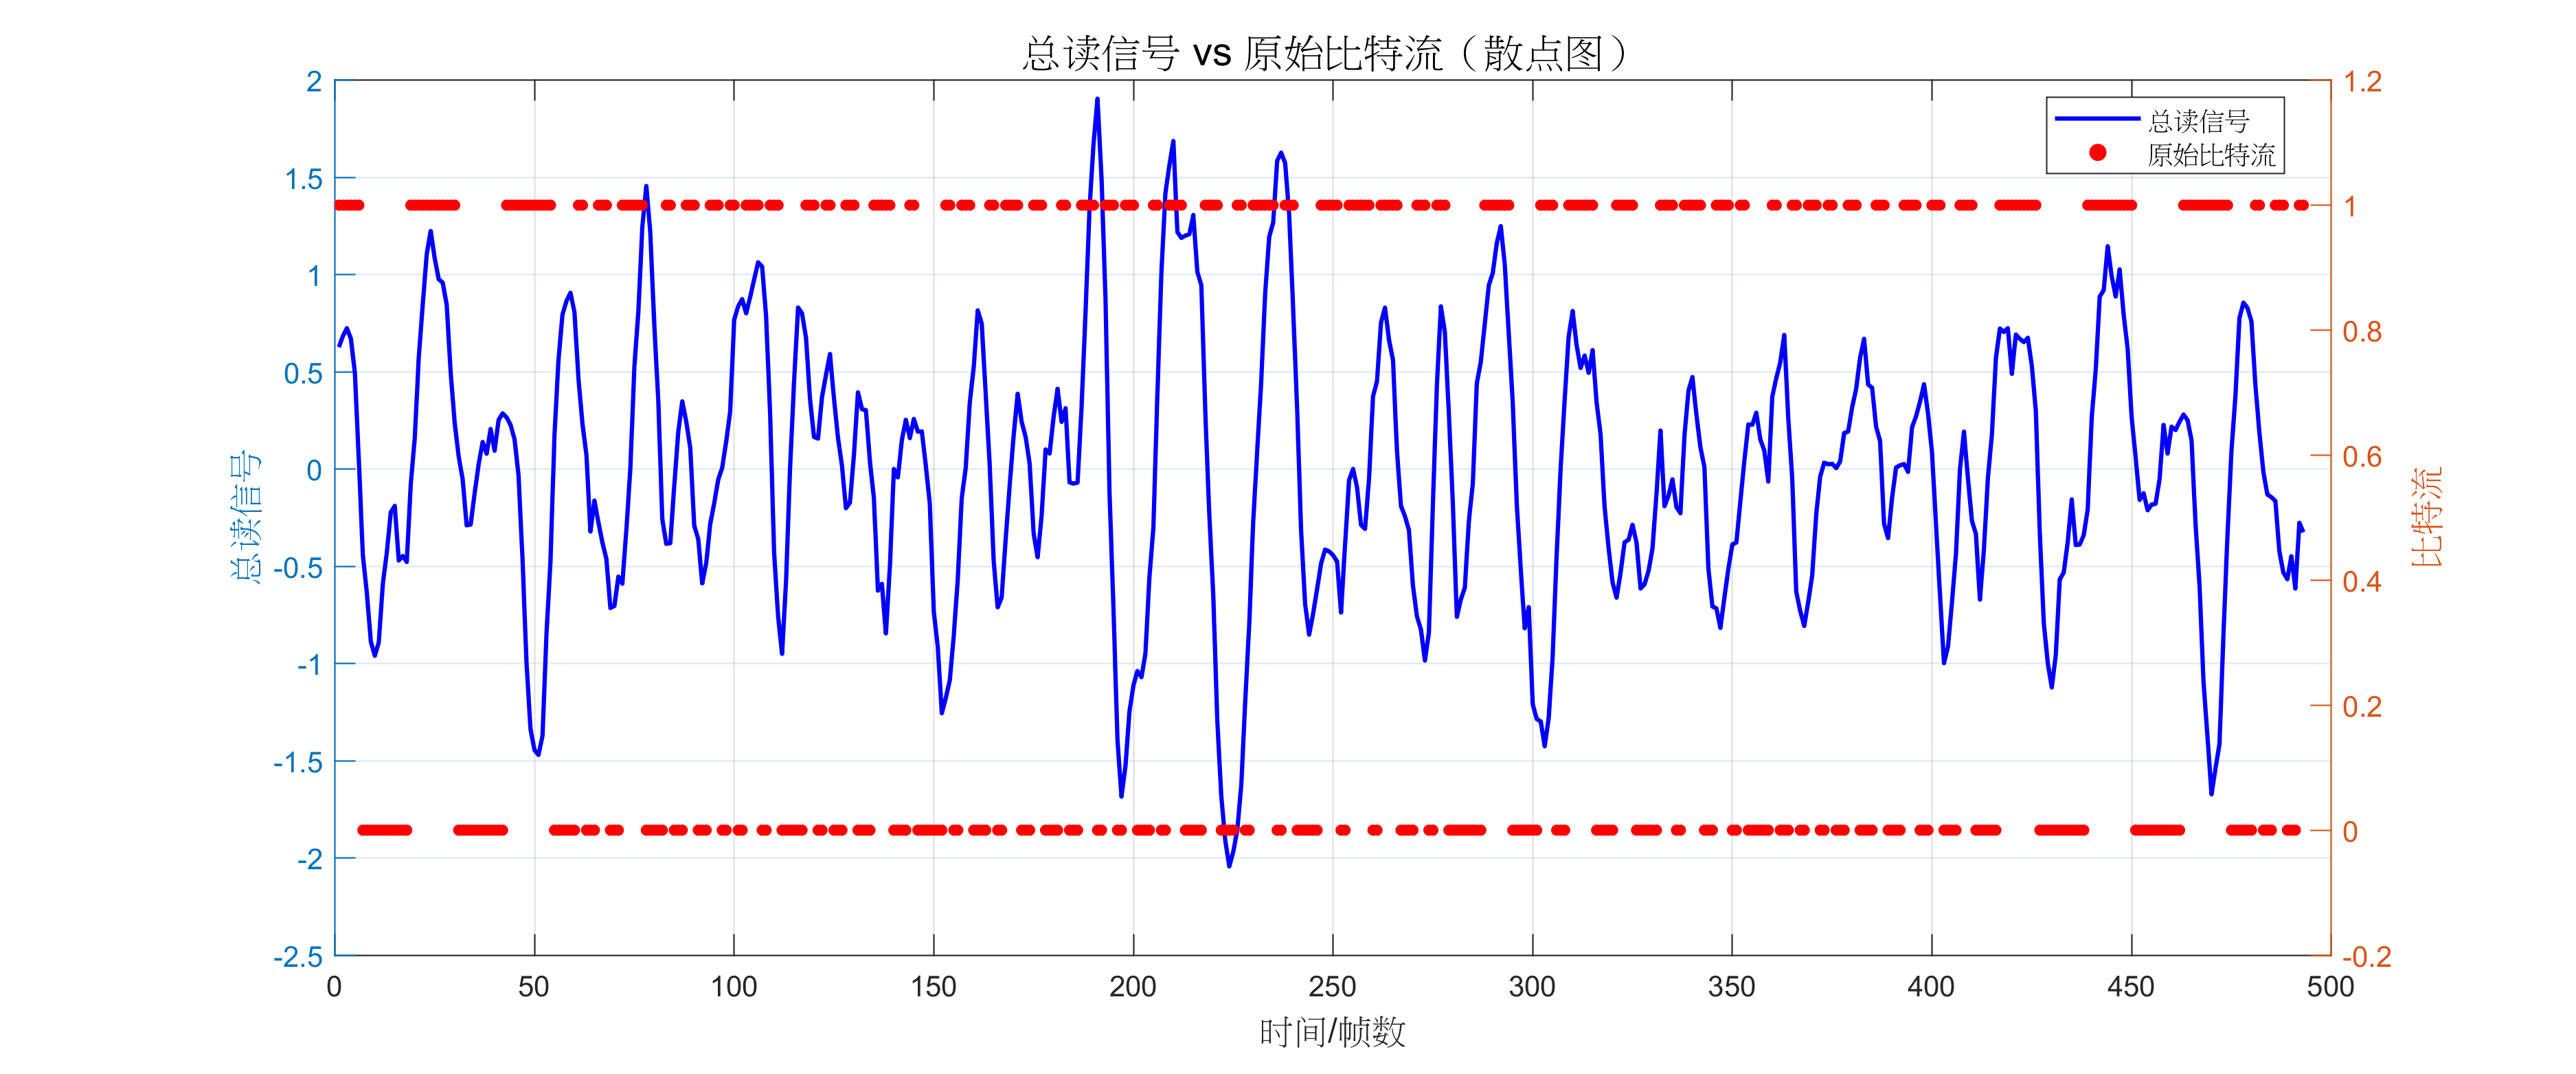
\includegraphics[width=\textwidth, trim=100 0 100 0, clip]{float/ch.cnn1/p1-shiye0-readdata-all.png}
	\caption{总回读信号与原始写入数据对比图\label{fig:ch.cnn1.readdata-all}}
\end{figure}

图\ref{fig:ch.cnn1.readdata-all}是总回读信号（A1+A2+B+D+E+F）与原始写入信号的对比图（展示前500个）。对比显示，尽管总信号大致跟随原始数据的包络，但存在明显的基线浮动与失真。特别是在连续跳变的信号附近，总回读信号并未保持平稳，而是出现了与相邻数据位相关的波动，这清晰地证实了道间串扰与符号间干扰的混合效应是客观存在且不可忽略的。单一的总和信号无法将来自目标轨道的有用信息与来自相邻轨道的干扰有效分离，其信噪比已难以满足更高密度存储的可靠性要求。

\begin{figure}[htbp]
	\centering
	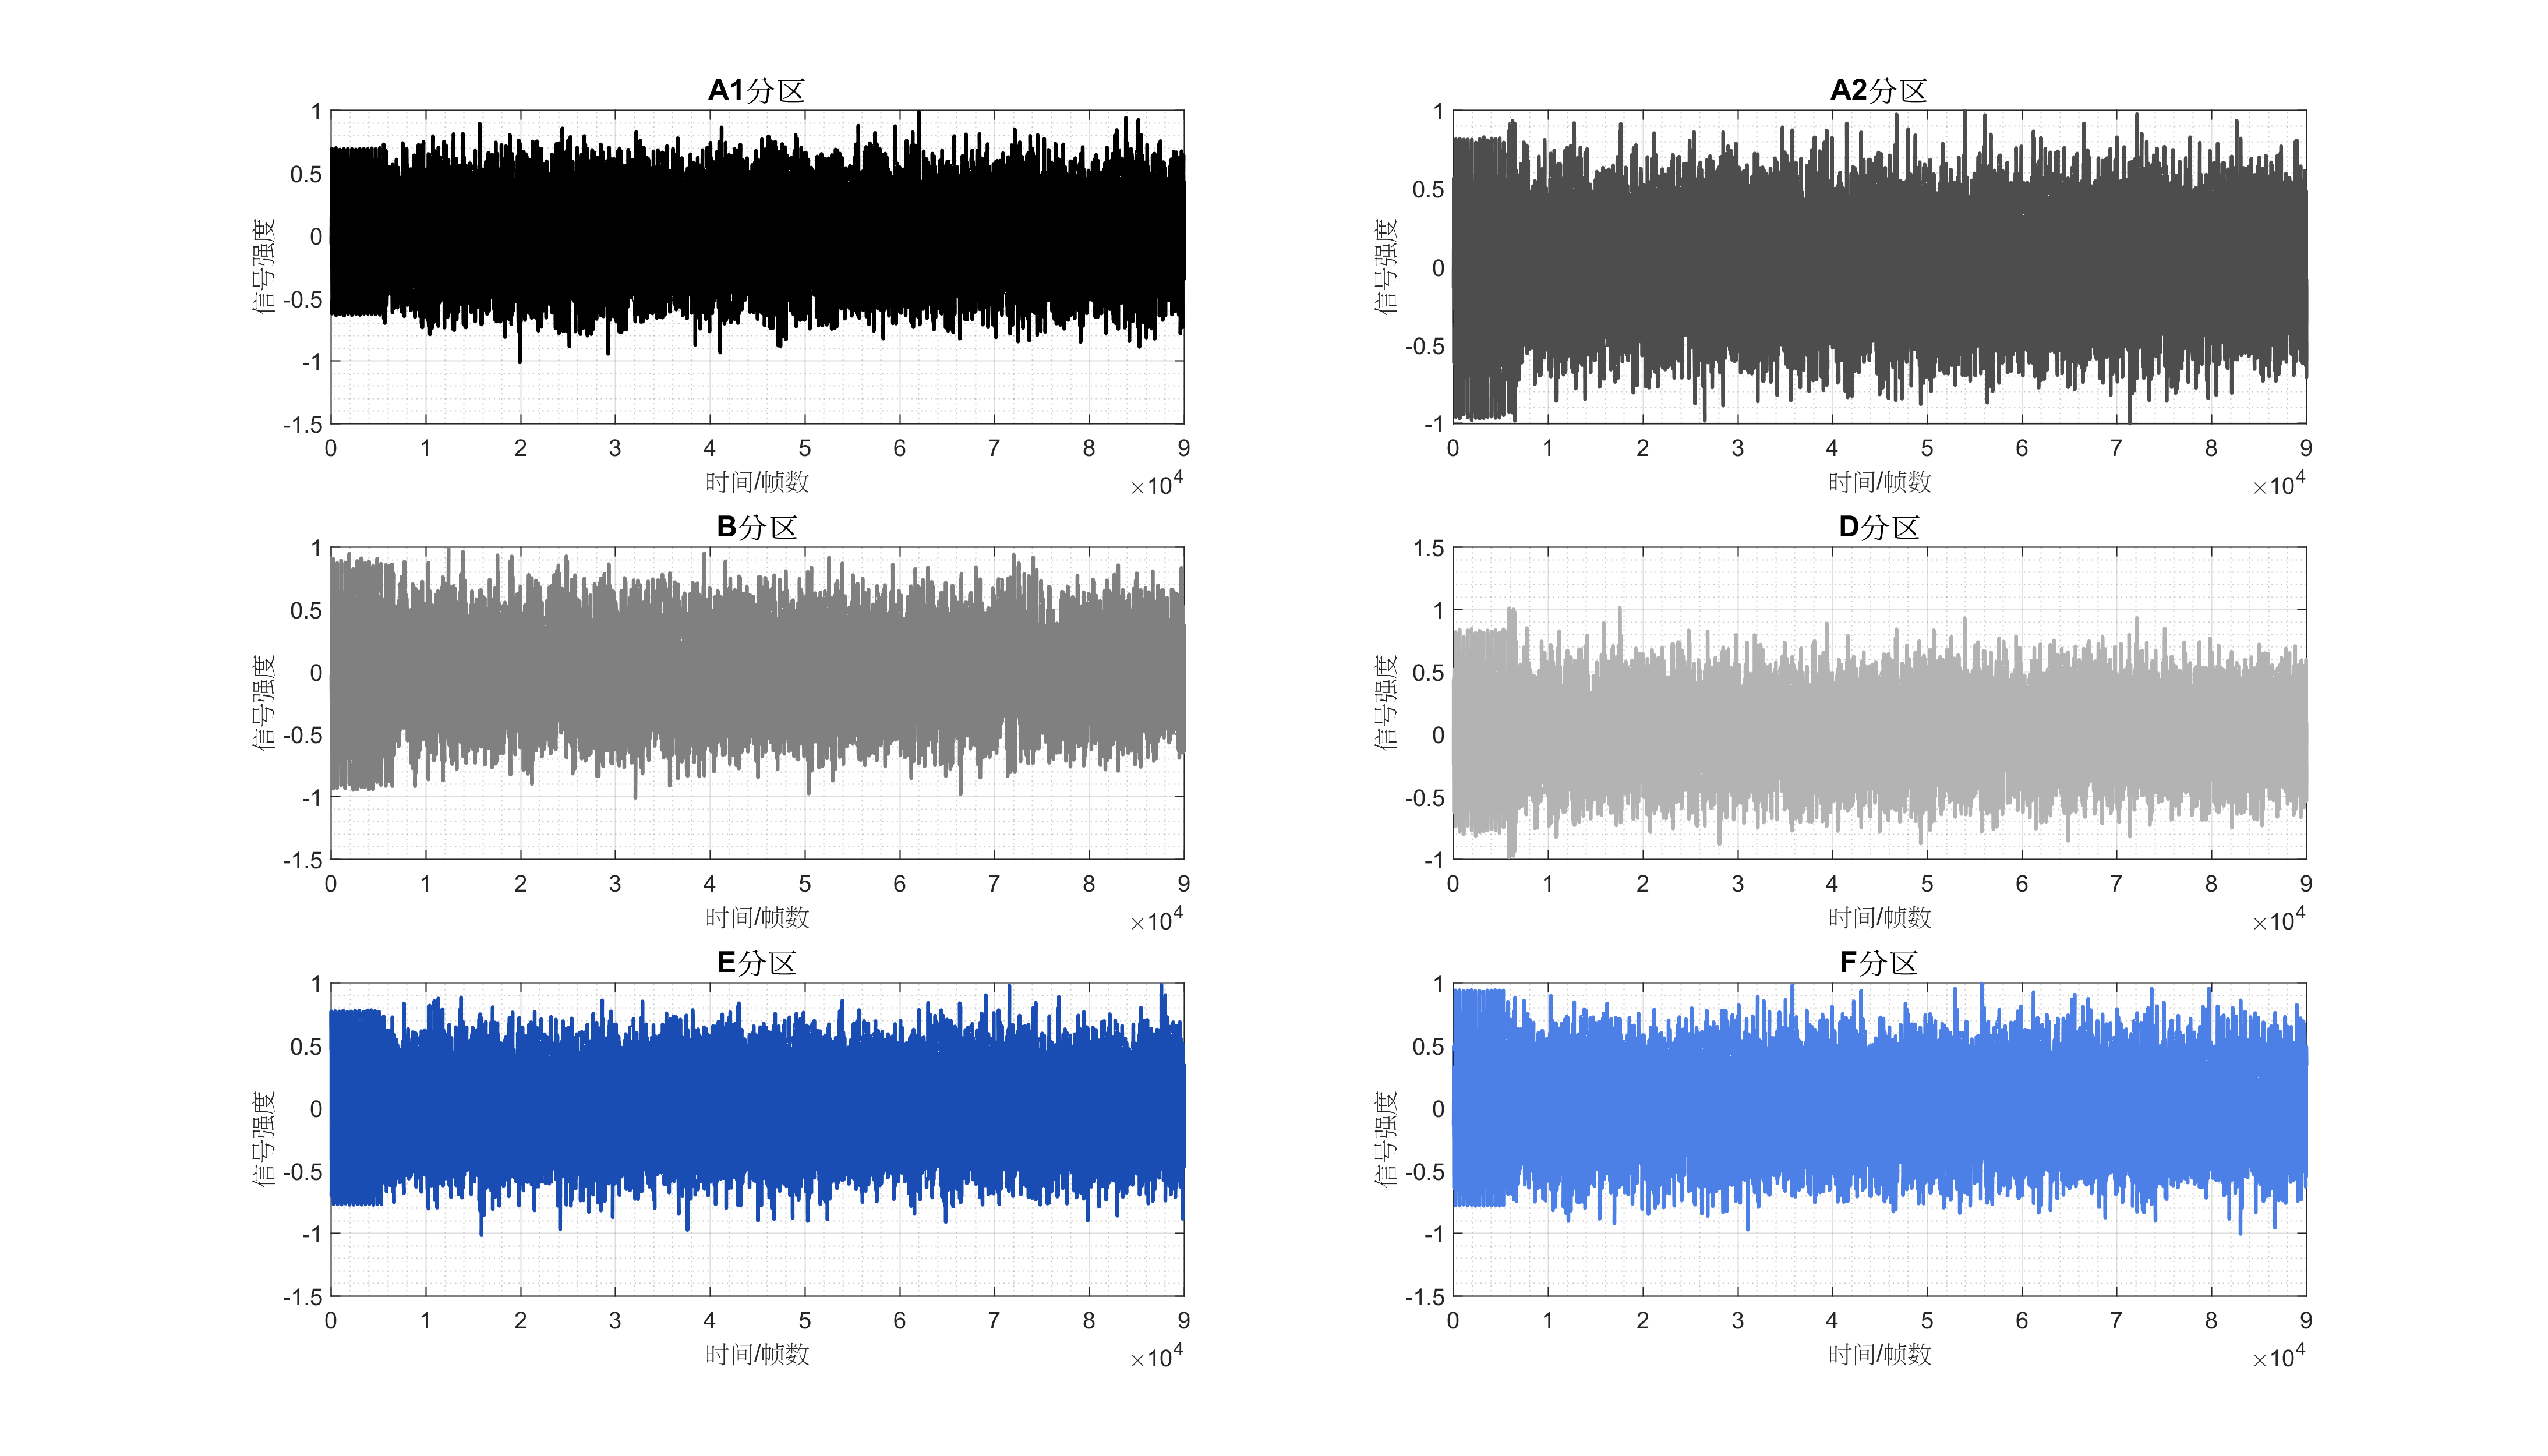
\includegraphics[width=\textwidth, trim=100 0 100 0, clip]{float/ch.cnn1/p1-shiye0-readdata.png}
	\caption{P1模式各分区回读信号对比图\label{fig:ch.cnn1.readdata}}
\end{figure}

图\ref{fig:ch.cnn1.readdata}展示了在上述条件下，添加了SA2umTilt0.2degDef0.2umDet60nmCNR复合噪声扰动后，P1分区模式下六个通道（A1, A2, B, D, E, F）生成的均衡前回读信号波形。六个通道的输出信号幅度存在显著差异。两侧通道（如 A1, A2）信号幅度波动差异最大，A2动态范围更宽，这是因为存在偏向于A2方向的噪声扰动，通过A2区域的光强更大。而位于光瞳外围的通道（如 E, F）信号幅度明显衰减，相比于A2分区，E、F分区的动态范围收窄，这与其主要接收来自PSF衍射环的较弱光强分布相符。


\section{本章小结}
本章针对高密度AD光盘均衡研究对信道模型的迫切需求，提出并构建了一种基于点扩散函数（PSF）的多分区信道建模方法。首先，分析了传统Bergmans简化模型与Braat-Hopkins严格物理模型在高精度与高效率之间难以兼顾的局限性。在此基础上，确立了以理想艾里斑PSF为核心、结合光学头分区几何特征的建模思路。借鉴TDMR系统的空间分集思想，对光学头分区策略进行了面向信号处理的优化设计，提出了P1分区模式，并构建了与之对应的多通道响应函数。最后，在典型AD500高密度参数下进行了仿真验证。结果表明，所生成的多通道信号（A1, A2, B, D, E, F）不仅直观反映了各分区在幅度与波形上的差异化特征，其总和信号也清晰地揭示出道间串扰与符号间干扰并存的实际信道状况，为后续章节利用多通道信号的空间特性进行联合检测与均衡提供了可靠的数据基础与模型支撑。本章工作为突破单一信道模型瓶颈、实现精准高效的信道仿真迈出了关键一步。